\documentclass[aspectratio=169]{beamer}
\mode<presentation>
{
    \usetheme{Boadilla}
    \usecolortheme{default}
    \usefonttheme{default}
    \setbeamertemplate{navigation symbols}{}
    \setbeamertemplate{caption}[numbered]
} 

\usepackage[magyar]{babel}
\usepackage[utf8]{inputenc}
\usepackage[T1]{fontenc}
\usepackage{graphicx, tikz, pgf, pgfplots}
\usepgfplotslibrary{polar}
\usepackage[framemethod=TikZ]{mdframed}


\newcommand\annotatedFigureBoxCustom[8]{
    \draw[#5,ultra thick,rounded corners] (#1) rectangle (#2);
    \node at (#4) [fill=#6,thick,shape=circle,draw=#7,
                   inner sep=2pt,font=\sffamily,text=#8]
                   {\textbf{#3}};
}


% {from}{to}{text}{color}
\newcommand\anbox[4]{\annotatedFigureBoxCustom{#1}{#2}{#3}{#1}{#4}{white}{black}{black}}


\newcommand\antext[5]{
    \draw[#4, fill=#5, ultra thick, rounded corners] (#1) rectangle (#2)
    node[pos=0.5, font=\sffamily, text=black] {\textbf{#3}};
}


\newenvironment{anfig}[1]
{
    \begin{mdframed}[linecolor=blue!65!white, linewidth=2pt, roundcorner=0.75pt,
                     innerrightmargin=0.05pt, innerleftmargin=0.05pt,
                     innertopmargin=0.05pt, innerbottommargin=0.05pt, frametitle={}]
    \begin{tikzpicture}
    \node[anchor=south west,inner sep=0] (image) at (0,0)
    {\includegraphics[width=\textwidth]{#1}};
    \begin{scope}[x={(image.south east)},y={(image.north west)}]
}
{
    \end{scope}
    \end{tikzpicture}
    \end{mdframed}
}

\def\rar{\rightarrow}
\def\lar{\leftarrow}


\newcommand\inc[1] {
    \includegraphics[width=\textwidth]{#1}
}

\newcommand{\ffig}[1]{
    \begin{mdframed}[linecolor=blue!65!white, linewidth=1.75pt, roundcorner=0.75pt,
                     innerrightmargin=0pt, innerleftmargin=0pt,
                     innertopmargin=0pt, innerbottommargin=0pt,
                     backgroundcolor=white, frametitle={}, align=center]
        \includegraphics[width=1.0\textwidth]{#1}
    \end{mdframed}
}


\newcommand\sepframe[1] {
    \begin{frame}
        \begin{center}
            \Huge \color{blue!55!black}
            #1
        \end{center}
    \end{frame}
}

%\newcommand\bench[2]{
    \begin{minipage}[t]{0.45\textwidth}
        \centering
        \includegraphics[width=\textwidth]{#1}
        \vspace{7.5pt}
        
        LOS deformáció.
    \end{minipage}
    \hspace{5pt}
    \begin{minipage}[t]{0.45\textwidth}
        \centering
        \includegraphics[width=\textwidth]{#2}
        \vspace{7.5pt}
        
        Kálmán-szűréssel integrált GNSS és InSAR mérések.
    \end{minipage}
}

\def\boxcolor{black}
\def\fillcolor{white}
\def\refcolor{orange}


\def\hun{
    \begin{anfig}{hungary_networks_raw.png}
        \anbox{0.27, 0.3}{0.33, 0.4}{A}{\boxcolor}
        \anbox{0.5, 0.4}{0.5525, 0.525}{B}{\boxcolor}
        \anbox{0.465, 0.05}{0.535, 0.15}{C}{\boxcolor}
    \end{anfig}
}

\def\erdely{
    \begin{anfig}{transylvania_networks_raw.png}
        \anbox{0.4075, 0.55}{0.4875, 0.67}{A}{\boxcolor}
        \anbox{0.55, 0.37}{0.63, 0.49}{B}{\boxcolor}
        \anbox{0.75, 0.08}{0.9, 0.4}{C}{\boxcolor}
    \end{anfig}
}

\def\dszekcso{
    \begin{anfig}{dszekcso_network_raw.png}
        \antext{0.05, 0.57}{0.25, 0.64}{IB1}{\refcolor}{\fillcolor}
        \antext{0.3, 0.67}{0.5, 0.74}{IB2}{\boxcolor}{\fillcolor}
        \antext{0.225, 0.47}{0.425, 0.54}{IB3}{\boxcolor}{\fillcolor}
        \antext{0.32, 0.25}{0.52, 0.32}{IB4}{\boxcolor}{\fillcolor}
    \end{anfig}
}

\def\kulcs{
    \begin{anfig}{kulcs_network_raw.png}
        \antext{0.125, 0.875}{0.225, 0.975}{A1}{\boxcolor}{\fillcolor}
        \antext{0.51, 0.45}{0.61, 0.55}{A2}{\boxcolor}{\fillcolor}
        \antext{0.825, 0.17}{0.925, 0.27}{A3}{\boxcolor}{\fillcolor}
        \antext{0.79, 0.04}{0.89, 0.14}{A4}{\boxcolor}{\fillcolor}
        \antext{0.46, 0.17}{0.56, 0.27}{AR}{\refcolor}{\fillcolor}
        \antext{0.475, 0.7}{0.625, 0.8}{Duna}{\boxcolor}{\fillcolor}
    \end{anfig}
}

\def\fonyod{
    \begin{anfig}{fonyod_network_raw.png}
        \antext{0.25, 0.78}{0.45, 0.86}{Balaton}{\boxcolor}{\fillcolor}
        \antext{0.725, 0.77}{0.825, 0.87}{KV}{\boxcolor}{\fillcolor}
        \antext{0.725, 0.16}{0.825, 0.26}{PH}{\refcolor}{\fillcolor}
        \antext{0.29, 0.0575}{0.39, 0.1575}{RE}{\boxcolor}{\fillcolor}
    \end{anfig}
}


\def\csomad{
    \begin{anfig}{ciomadul_network_raw.png}
        \antext{0.3, 0.29}{0.42, 0.375}{C1}{\boxcolor}{\fillcolor}
        \antext{0.21, 0.1}{0.33, 0.18}{C2}{\refcolor}{\fillcolor}
        \antext{0.665, 0.2}{0.775, 0.28}{C3}{\boxcolor}{\fillcolor}
        \antext{0.49, 0.565}{0.6, 0.645}{C4}{\boxcolor}{\fillcolor}
        \antext{0.64, 0.82}{0.76, 0.9}{C5}{\refcolor}{\fillcolor}
    \end{anfig}
}


\graphicspath{{../../images/}}

\title[Műholdas Távérzékelés Labor, 2018/19.I.]{Műholdas Radar Interferometria elmélete és alkalmazásai}
\author[Bozsó István]{Bozsó István}
\institute[MTA CSFK GGI]{MTA CSFK Geodéziai és Geofizikai Intézet}
\date{2018.12.13.}


\begin{document}

\begin{frame}
    \titlepage
    \begin{center}
        \begin{minipage}[c]{0.3\textwidth}
            \includegraphics[width=0.75\textwidth]{ggi_logo.png}
        \end{minipage}
    \end{center}
\end{frame}

\begin{frame}{Áttekintés}
    \tableofcontents
\end{frame}

\def\ft{Ismétlés - Szintetikus Apertúrájú Radar}
\section{\ft}


\begin{frame}{\ft}
    \begin{itemize}
        \item kiváló térbeli felbontás, egy csatornán (mikrohullámú tartomány)
        \begin{itemize}
            \item L-sáv: 1-2 GHz; 30-15 cm (PalSAR)
            \item S-sáv: 2-4 GHz; 15-7.5 cm
            \item C-sáv: 4-8 GHz; 7.5-3.8 cm (Sentinel-1, ERS, Envisat)
            \item X-sáv: 8-12 GHz; 3.82.5 cm (TerraSAR-X)
        \end{itemize}
        \item koherens radar: amplitúdó ÉS fázis regisztrálása
        \item alkalmazás amplitúdóra: Freidl Zoli előadása
    \end{itemize}
\end{frame}


\begin{frame}{\ft}
    % \cite{RamonHanssen}
    \begin{figp}{ramon_SAR.png}{Radar felvétel geometriája}{0.5}{0.4}
        RAR (Real Aperture Radar) felbontása: azimut / slant range $\approx 5$ km, ground range $\approx 14$ km:
        $$ \subt{W}{a} = \frac{\lambda}{\subt{L}{a}} R $$
        $$ \subt{\Delta}{r} = \frac{c\tau}{2} $$
    \end{figp}
\end{frame}

\def\ft{Range felbontás növelése}
\subsection{\ft}

\begin{frame}{\ft}
    \begin{figp}{chirp_demod.png}{}{0.4}{0.4}
        Chirp jel kibocsájtása, visszavert jel feldolgozása illesztett szűréssel:
        \begin{align*}
            f(t) &= a t & \text{lineárisan növekvő frekvencia} \\
            \subt{B}{R} &= a \tau & \text{sávszélesség} \\
            \subt{\Delta}{r} &= \frac{c}{2 \subt{B}{R}} \approx 9.6 m & \text{slant range felbontás}
        \end{align*}
        $\approx 25$ m ground range felbontás
    \end{figp}
\end{frame}

\def\ft{Azimut felbontás növelése}
\subsection{\ft}

\begin{frame}{\ft}
    \begin{center}
    \begin{minipage}[c]{0.45\textwidth}
        \fig{sar_synthetic_length.png}
    \end{minipage}
    \hspace{10pt}
    \begin{minipage}[c]{0.45\textwidth}
        \fig{chirp_azimuth.png}
    \end{minipage}
    \end{center}
\end{frame}


\def\ft{Nyers SAR felvétel fókuszálása}
\subsection{\ft}

\begin{frame}{\ft}
    \begin{minic}{0.8}
        \inc{rng_azi_compression.png}
        
        \centering
        Felbontás fókuszálás után: ground range: $\approx 25$ m, azimut: $\approx 10$ m (ERS-1,2)
    \end{minic}
\end{frame}


\def\ft{Ismétlés - Szintetikus Apertúrájú Radar}

\begin{frame}{\ft}
    \begin{minic}{0.85}
        \inc{mw_bands.png}
        
        \centering
        Különböző radarsávban készült felvételek egy területről.
    \end{minic}
\end{frame}


\begin{frame}{\ft}
    % insartut
    \begin{figp}{sar_speckle.png}{}{0.45}{0.45}
        \begin{itemize}
            \item amplitúdó ÉS fázis érték pixelenként; komplex számként reprezentálható
            \item $\subt{C}{SAR} = A e^{i\phi}$
            \item $\subt{C}{SAR} = \sum_j c_{\text{SAR},j}$
            \item 
        \end{itemize}
    \end{figp}
\end{frame}

\begin{frame}{Egy hullám fázisa}
    \newcommand{\sinPhase}[2] {
    \addplot[smooth, domain=0:360,line width=1.5pt, #2]{sin(x - (#1))};
}

\newcommand{\phase}[2] {
    \addplot[->, >=latex, line width=2.5pt, #2] coordinates { (0,0) (#1,1.5) };
}

\begin{center}
\begin{tabular}{rl}
\begin{tikzpicture}[baseline,scale=0.9]
\begin{axis}[
    domain=0.0:360,
    xlabel={$x$ (deg)},
    ylabel={$y = f(x)$},
    enlarge x limits=false,
    legend style={at={(0.5, -0.2)}, anchor=north, legend columns=3},
]
    \sinPhase{0}{blue}
    \sinPhase{90}{red}
    \sinPhase{210}{green}
    \legend{$\sin(x)$, $\sin(x - 90^\circ)$, $\sin(x - 210^\circ)$}
\end{axis}
\end{tikzpicture}
&
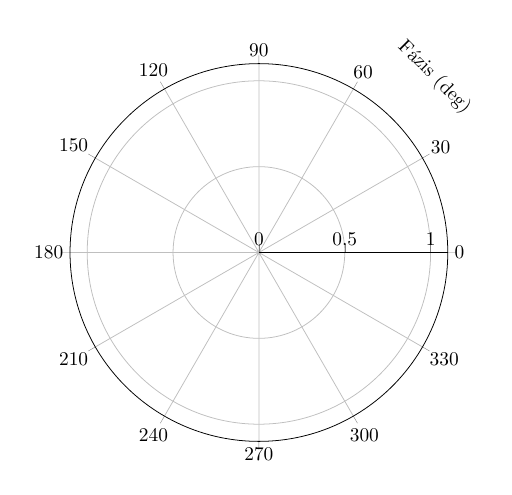
\begin{tikzpicture}[baseline,scale=0.7]
\begin{polaraxis} [
    xlabel={Fázis (deg)},
    ytick = \empty,
]
    \phase{0}{blue}
    \phase{90}{red}
    \phase{210}{green}
\end{polaraxis}
\end{tikzpicture}
\end{tabular}
\end{center}

\end{frame}


\begin{frame}{Egy SAR felvétel fázisképe}
    \begin{minic}{0.5}
        \figc{vrancea.png}{Asd}
    \end{minic}
\end{frame}


\begin{frame}{\ft}
    Goldstein-szűrés:
    \[
        H(u,v) = Z(u,v) \abs{Z(u,v)}^{\alpha}
    \]
    \begin{itemize}
        \item $H(u,v)$: szűrt értékek
        \item $Z(u,v)$: eredeti értékek
        \item $\alpha$: szűrés erőssége; $\alpha = 0$ nincs szűrés
    \end{itemize}
\end{frame}

%\bibliography{../../insar}

\end{document}
